\documentclass[10pt,a4paper]{article}


% Packages laden
\usepackage[a4paper,top=3cm,bottom=2cm,left=2cm,right=2cm]{geometry}		% paginagrootte
%\usepackage{a4wide}
\usepackage{parskip}									% andere regels voor nieuwe paragraaf: witregel + niet inspringen

\usepackage[english]{babel}						%	spelling en woordafbreking (Engels)
\usepackage[latin1]{inputenc}					% invoer van speciale tekens (bvb. Umlaut)
\usepackage[T1]{fontenc}							% weergave van speciale tekens (bvb. Umlaut)
\usepackage{lmodern}									% betere weergave van speciale tekens (bvb. Umlaut)
%\usepackage{dsfont}	
\usepackage{amsfonts,amsthm, tabularx}					% wiskundige symbolen and table of equations
%\usepackage[fleqn]{amsmath}
\usepackage{graphicx}
\usepackage{epstopdf}

% Package for hyperlink, without ugly box around and nice blue color for text
\usepackage{hyperref}
\usepackage{xcolor}
\hypersetup{
    colorlinks,
    linkcolor={red!50!black},
    citecolor={blue!50!black},
    urlcolor={blue!80!black}
}

\usepackage{graphicx}
\usepackage{caption}
\usepackage{subcaption}

\usepackage{float}										% plaatsen van figuren en tabellen
\usepackage[format=plain,
						indent=1cm]{caption}			% personaliseren van onderschriften
\usepackage{eurosym}									% sign of euro

% Instellingen voor document
\renewcommand{\arraystretch}{1.1}			% tabelrijen iets hoger maken

\usepackage{amsmath,amsfonts,amsthm,mathrsfs,MnSymbol}	% wiskundige symbolen
\renewcommand*\thesection{\arabic{section}}
\DeclareMathOperator*{\argmin}{\arg\!\min}
\usepackage{pifont}							

\setcounter{secnumdepth}{3}		% Enable subsubsection numbering
\setcounter{tocdepth}{3}		% Include subsubsection in table of content

\usepackage{color}				% Load the color package: \color{declared-color}{text}. If also background:
								% \colorbox{declared-color1}{\color{declared-color2}text}
%Aangepaste header
\usepackage{fancyhdr}
\pagestyle{fancyplain}
\renewcommand{\headrulewidth}{1.0pt}
\lhead{\fancyplain{}{Crash course Modelica}}
\rhead{\fancyplain{}{\today}}

\usepackage{listings}
\usepackage{siunitx}
%% listings-modelica.cfg
%% Copyright 2014 Martin Sjoelund, Dietmar Winkler
%
% This work may be distributed and/or modified under the
% conditions of the LaTeX Project Public License, either version 1.3
% of this license or (at your option) any later version.
% The latest version of this license is in
%   http://www.latex-project.org/lppl.txt
% and version 1.3 or later is part of all distributions of LaTeX
% version 2005/12/01 or later.
%
% This work has the LPPL maintenance status `maintained'.
%
% The Current Maintainer of this work is Dietmar Winkler
%
% Code repository https://github.com/modelica-tools/listings-modelica
%
% This work consists of the file listings-modelica.cfg

\lstdefinelanguage{modelica}
{
  morekeywords=[1]{
    algorithm,and,annotation,as,assert,block,break,case,class,connect,connector,
    constant,constrainedby,der,discrete,each,else,elseif,elsewhen,encapsulated,
    end,enumeration,equality,equation,expandable,extends,external,failure,final,
    flow,for,function,guard,if,import,in,initial,inner,input,List,local,loop,
    match,matchcontinue,model,not,operator,Option,or,outer,output,package,parameter,
    partial,protected,public,record,redeclare,replaceable,return,stream,
    subtypeof,then,Tuple,type,uniontype,when,while},
  morekeywords=[2]{true, false},
  % Do not make true,false keywords because fn(true,x, false ) shows up as fn(true,x, *false*)
  morekeywords=[3]{optimization,constraint}, % Optimica keywords
  morekeywords=[4]{objective,startTime,finalTime,initialGuess},
  sensitive=true,
  comment=[l]//,
  morecomment=[s]{/*}{*/},
  alsodigit={.,-},
  morestring=[b]',
  morestring=[b]",
}[keywords,comments,strings]

\definecolor{keywordcolor1}{rgb}{0,0,.4}
\definecolor{keywordcolor2}{rgb}{.90,0,0}
\definecolor{keywordcolor3}{rgb}{.4,0,.8}
\definecolor{keywordcolor4}{rgb}{0.5,0,0.5}
\definecolor{stringcolor}{rgb}{0.133,0.545,0.133}
% \definecolor{listingbgcolor}{rgb}{0.95,0.95,0.95}

\lstset{
  breaklines=true,
  language=modelica,
  basicstyle=\ttfamily,
  keywordstyle=[1]\color{keywordcolor1}\bfseries,
  keywordstyle=[2]\color{keywordcolor2},
  keywordstyle=[3]\color{keywordcolor3}\bfseries,
  keywordstyle=[4]\color{keywordcolor4},
  stringstyle=\color{stringcolor},
%  backgroundcolor=\color{listingbgcolor},
  framexleftmargin=5pt,
  xleftmargin=5pt,
  xrightmargin=5pt,
  showstringspaces=false
}

\newcommand{\code}[1]{\lstinline|#1|}
\newcommand{\modelica}[1]{\lstinline[language=modelica]|#1|}


\usepackage{color}

\definecolor{backcolour}{rgb}{0.95,0.95,0.92}

\lstset{language = modelica,
	backgroundcolor = \color{backcolour}}

\usepackage[scaled]{beramono}
\usepackage[T1]{fontenc}
\usepackage{todonotes}

\author{Bram van der Heijde}
						
\begin{document}
	
	\title{Prepare for the Modelica Crash Course!}
	\author{Filip Jorissen, Damien Picard, Jelger Jansen, Iago Cupeiro Figueroa} 
	\date{KU Leuven -- September 13, 2022}
	\maketitle

This guide will help you to install Dymola and already get the hang of Modelica, such that you can profit maximally from the crash course. 

\subsection*{Installation}

\begin{enumerate}
	\item First of all, install Dymola (commercial software).  Download the trial version on
	\href{https://www.3ds.com/products-services/catia/products/dymola/trial-version/}{this page}. You will be able to use a license from our license pool during the crash course. 
	\item After installation you \textbf{have} to install a C compiler, otherwise you 
	cannot simulate any model. We can suggest to use \href{https://visualstudio.microsoft.com/fr/vs/older-downloads/}{Visual Studio 2019}, but other compilers are possible as well. For detailed instructions see
	\href{http://www.Dymola.com/compiler}{http://www.Dymola.com/compiler}. 
	\item Do not forget to select your C compiler in \texttt{Simulation>Set Up>Compiler}. In order to access this menu item, open Dymola and change to the Simulation tab (tab bar at the top).
	\item Test your installation by running a demo (e.g. open \texttt{File>Demos>Robot}, then 
	click \texttt{Simulation> Simulate} and wait till you see a graph). More detailed instructions can be found \href{https://www.3ds.com/fileadmin/PRODUCTS/CATIA/DYMOLA/PDF/Installation.pdf}{here}.
\end{enumerate}


\subsection*{Optional preparation material}
To get the most out of the crash course, we suggest to come prepared by installing Dymola (which occasionally takes some time) and making a preparatory homework exercise, which can be found below. 

We also suggest to read the following chapters of the open-access book \href{https://mbe.modelica.university/}{Modelica by Example} by M. Tiller carefully.

\begin{enumerate}
\item \href{https://mbe.modelica.university/behavior/equations/}{Basic equations}: General introduction to the Modelica language, illustration of the model structure, basic concepts such as derivative, initialization, parameter, variable and type.
\item \href{https://mbe.modelica.university/behavior/functions/polynomial/}{Polynomial 
Evaluation}: Example of \href{https://mbe.modelica.university/behavior/functions/func_def/}{function definition}, protected variable and time.
\item \href{https://mbe.modelica.university/behavior/arrays/oned/}{One-Dimensional Heat Transfer}: Introduction to arrays and loop in Modelica.
\item \href{https://mbe.modelica.university/components/connectors/}{Connectors}: Component-oriented modeling, classes of variables.
\end{enumerate}

Additionally, we stronly recommend to read Chapter 1 ``What is Dymola?'' (p.~9-20) of the Dymola User Manual. This chapter gives more information on the features of Dymola and Modelica and explains the Dymola environment (graphical user interface, model editor, parameters change, simulation, ...). The Dymola User Manual can be found in your installation folder of Dymola: \texttt{C:\textbackslash Program 
Files (x86)\textbackslash Dymola \textit{xx}\textbackslash Documentation 
\textbackslash Dymola User Manual 1A}, where \textit{xx} stands for the 
version you installed. 

For further background, the following sections from ``Modelica by Example'' by 
M. Tiller are interesting. However, it is not required to read before the 
course: 

\begin{enumerate}
\item \href{https://mbe.modelica.university/behavior/discrete/}{Discrete Behavior}: State event handling and hysteresis.
\item \href{https://mbe.modelica.university/behavior/arrays/}{Vectors and Arrays}: Array declarations and array construction
\item \href{https://mbe.modelica.university/components/components/}{Components}: Syntax, arguments and examples (e.g. heat transfer and electrical components).
\item \href{https://mbe.modelica.university/components/architectures/}{Architecture}: Configuration management.
\end{enumerate}

Finally, the \href{https://modelica.org/documents/MLS.pdf}{Modelica Language Specification} is a complete description of the Modelica language.

\subsection*{Homework exercise}
Consider the electrical circuit shown in Fig.~\ref{fig:cir}. The circuit has a sinusoidal source, two resistors, a diode, a capacitor and the ground. The purpose of this exercise is to learn some basic Modelica concepts by creating the model of this electrical circuit from scratch. You will learn how to create connectors, partial models and models and how to re-use your code.

\begin{figure}[h]
	\centering
	\begin{minipage}{.4\textwidth}
		\centering
		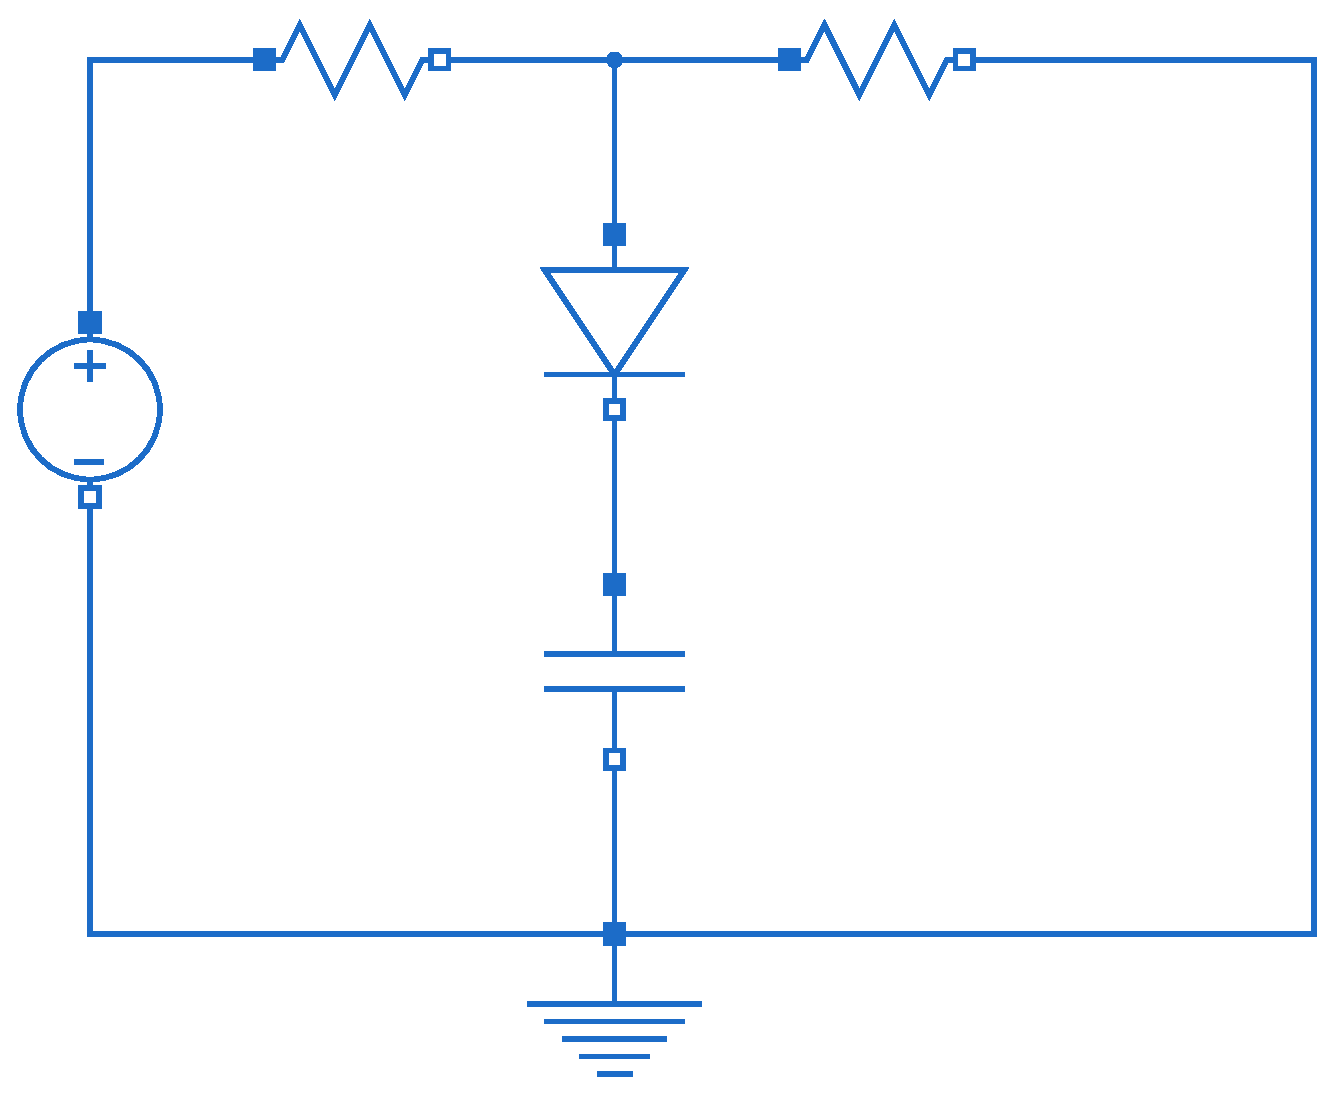
\includegraphics[width=1\linewidth]{images/circuit.eps}
		\captionof{figure}{Electrical circuit}
		\label{fig:cir}
	\end{minipage}%
	\begin{minipage}{.6\textwidth}
		\centering
		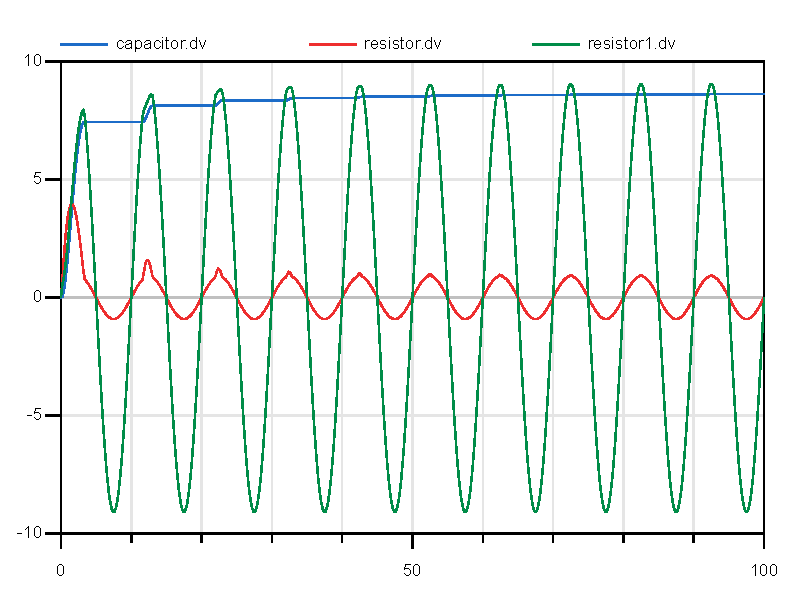
\includegraphics[width=.8\linewidth]{images/result.eps}
		\captionof{figure}{Result of simulation}
		\label{fig:res}
	\end{minipage}
\end{figure}
\vspace{3 mm}
Some tips:
\begin{itemize}
	\item Make sure you end statements in Modelica code with a semicolon (\textbf{;}). With some exceptions (e.g., \texttt{(partial) model}, \texttt{equation} and \texttt{algorithm} lines), this is always necessary.
	\item You can check your model using the \texttt{check} button in the toolbar. This will usually point you to possible mistakes you made, so make sure to read error and warning messages carefully. Although Modelica has a bad reputation for debugging, its syntax checker is not bad.
	\item Dymola has a nifty autocompletion function, which helps you reduce how much of the code you have to type yourself. Just start typing something and press \texttt{Ctrl+space} to open a context menu with some suggestions.
\end{itemize}
\vspace{5 mm}

Below you can find a more detailed procedure in order to get a simulation model of the electrical circuit. Summarised, you will start by making a new library (package). In that package you will define an electrical connector in which the current and voltage are declared as variable. Then, you will create a positive and negative pin by extending the general electrical connector. Subsequently, the positive and negative connector can be used to define a partial model that describes any electrical component with two connectors. This partial model can be extended in a next step to create customised electrical components (resistor, capacitor, ...). Once you have made these models, you can build and simulate the electrical circuit shown in Fig. \ref{fig:cir}.
\vspace{5 mm}

\begin{enumerate}
	\item After opening Dymola, create a new \textit{package} called \textit{MyLib} (through \texttt{File>New>Package}). Don't forget to provide an appropriate description so you know what your library is for when you don't touch it for a longer time. It is useful to deselect ``Save contents of package in one file'' if you are going to use version control (git).
	
	All component models you will define in the following step need to be placed in this folder.
	
	\item Each component uses electrical connectors. Create a \texttt{partial connector} (right-click \textit{MyLib}, then \texttt{New> Connector}). Make sure to select the option ``Partial'' in the dialog that pops up. Call the \texttt{partial connector} \textit{Pin}. This connector will need two variables: $i$ (current) and $v$ (voltage). You can add variables while you are in the \textit{text editor} of Dymola (\texttt{Text>Modelica Text}). If you want to know how to create variables in the text editor, you can review \href{https://mbe.modelica.university/behavior/equations/variables/#variables}{this page}. 

	Which one is a \textit{flow} variable and which one is a \textit{potential} variable, and how should this be reflected in your code? Check 
	\href{https://mbe.modelica.university/components/connectors/simple_domains/#simple-domains}{this link} for a hint.
	
	\item Create the \texttt{connector}s \textit{Pin\_a} and \textit{Pin\_b} for the positive and negative pins. Use \texttt{extends} to inherit the variables $i$ and $v$ from the \texttt{partial connector} you have just defined. An easy way to create extending models is by right-clicking on the model you want to extend from, and click \texttt{New>Extend from}.
	
	Make two different graphical illustrations for the pins. To do so, select the \textit{icon context} from the toolbar (\texttt{Graphics>Icon}). For example, you can draw a square in the available canvas and choose a different color for each of the pins. A good convention is to use the same shape for pins of the same flow type. 
	
	\item Create a \texttt{partial model} \textit{OnePin} which contains the variables $i$ (current) and $v$ (voltage) and one connector \textit{Pin\_a}. To add the connector, drag \textit{Pin\_a} from your libary folder to the modelling window while you are in the \textit{diagram context} (\texttt{Graphics>Diagram}). The pin should be located on the top border of the white canvas. This model will be the basis for all models which have only one pin (i.e. the ground node).
	
	\item Create variables $i$ and $v$ in \textit{OnePin} and write \texttt{equation}s to link these variables to those you have defined in the \textit{Pin} you use in the component. In order to access variables, you can use dot notation as follows: \texttt{componentName.variable}.
	
	Your code should look something like this:
	\begin{lstlisting}
	partial model OnePin "Model with a single pin"
	  flow Modelica.Units.SI.Current i "Current flowing through this component";
	  Modelica.Units.SI.Voltage v "Voltage of this component";
	
	  Pin_a pin annotation...;
	equation
	  pin.i = i;
	  pin.v = v;
	  annotation...;
	end OnePin;
	\end{lstlisting}

	Notice that the model \texttt{OnePin} contains an instance of \texttt{Pin\_a} named \texttt{pin}. In the \texttt{equation} section, you can see that the current through this \texttt{pin} is accessed with the dot-notation and made equal to the current of the \texttt{OnePin}. The same is done for the voltages.
	
	However, it is not possible to access a variable on something that is not an instance of a Modelica model. For instance, \texttt{OnePin.v} would make no sense.
	
	\item Now create a \texttt{partial model} \textit{TwoPin} with the same variables and two \textit{Pin} connectors, one positive pin on the left and one negative on the right. Add two variables: voltage difference between the two pins $dv$ and current $i$. 
	
	While still in \texttt{partial model} \textit{TwoPin}, add equations that link the variables in this model with the variables of the pins. When connecting currents, use the convention that when the current flows into the component from the pin, it is positive and vice versa.
	
	\item Create the models for the source, the resistor, the diode and the capacity by extending \textit{OnePin} or \textit{TwoPin}. Make use of the following equations:
	\begin{enumerate}
		\item Resistor: $R i = v$\footnote{$v$ in this equation is equivalent to variable $dv$ in the Modelica model.}
		\item Capacity: $C \frac{d v}{dt} = i$
		\item Source: $v = V sin( 2 \pi f t + \omega) + \beta$
		\item Diode: if $ \frac{v}{V_t} \geq \alpha$: $i = I_{ds} \left( \exp\left(\alpha \left( 1 + \frac{v}{V_t} - \alpha \right)\right) - 1\right) + \frac{v}{R}$, else $i = I_{ds} (e^\alpha - 1) + \frac{v}{R}$
		\item Ground: $ v = 0$
	\end{enumerate}
	Define the constants $R$, $C$, $V$, $\ldots$  as \texttt{parameter}, such that you can change their value using the parameter dialog in the \textit{Diagram} context.
	
	To review how to define the time derivative of a variable, revise 
	\href{https://mbe.modelica.university/behavior/equations/first_order/}{this link}.
	\item Create a model called \textit{Circuit} in which you include all these components as shown in Fig.~\ref{fig:cir}. 
	
	You are very welcome to experiment with model parameters, but to verify your solution against Fig.~\ref{fig:res}, use following parameters:
	\begin{itemize}
		\item Voltage source: $f =$ \SI{0.1}{\hertz}, $V =$ \SI{10}{\volt}
		\item Left resistance: $R =$ \SI{1}{\ohm}
		\item Right resistance: $R =$ \SI{10}{\ohm}
		\item Diode: $I_{ds}$ = 1.e-6, $V_t=0.04$, $\alpha=1$, $R=1.e8$.
		\item Capacitor: $C =$ \SI{1}{\farad}, $V_0 =$ \SI{0}{\volt} (start voltage)
	\end{itemize}
	\item Simulate the circuit for 100 seconds.
\end{enumerate}

\vspace{15 mm}

\subsection*{Optional exercise}
This assignment aims at testing your comprehension of the basic Modelica concepts learned during the above mentioned reading by setting a model of a building and simulating its thermal behaviour. \textbf{This assignment will not be treated during the Crash Course.} However, you may find it a useful exercise to get more acquainted with Modelica and Dymola.

Let us consider a simplified building as represented in Fig. \ref{fig:bui}. The building consists of a single room called \textit{zone}, walls, a floor (foundation), a roof and a window. The building thermally interacts with the environment: ambient air (\textit{TAmb}), the ground, and the sun (\textit{QSol}). The building foundation is approximated by a thick concrete layer called \textit{slab} separating the zone from the ground. 

On the right-hand side of the figure, a thermal model of the building is proposed using the resistance-capacitance approach. The heat transfer through the building envelope is approximated by a 1D heat flow (conduction) through equivalent thermal resistances. The thermal storage in the building envelope, due to its thermal inertia, is approximated by equivalent thermal capacities. \textit{CZone} represents the thermal capacity of the zone (consisting of the internal walls, the furnitures, and a part of the external wall). The \textit{CSlab} represents the thermal capacity of the slab. Finally, the ground is discretized in \textit{n = 5} layers, each of them having an identical heat capacity \textit{CGro[i]}. Through the window, the sun heats up the room with a thermal power $QSol$. 
\vspace{15 mm}

\begin{figure}[h] 
	\centering
	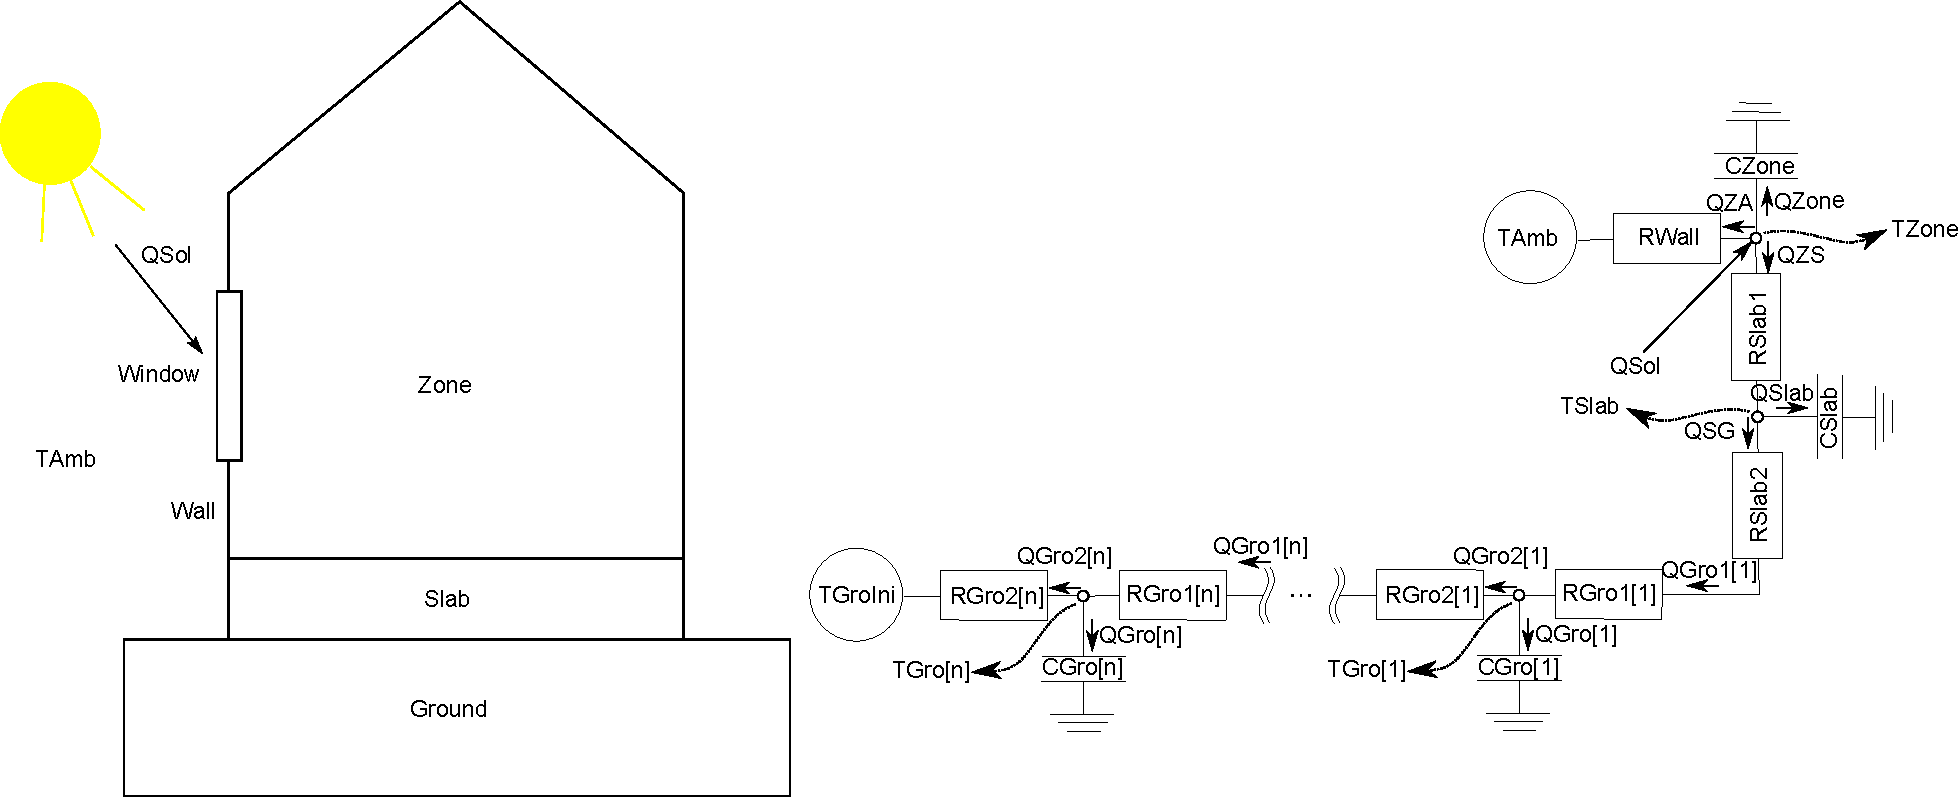
\includegraphics[width=1 \textwidth]{images/RCModelHouse.pdf}
	\caption{ Building model.}
	\label{fig:bui}
\end{figure}


The values of the parameters are given in Table \ref{tab:par}. Using the electrical analogy, the governing equations of the system are the following:

\textbf{Thermal resistance}: $T_1 - T_2 = \text{R} \ Q_{1 \rightarrow 2} $ with $R$ the thermal resistance between node 1 and 2 and $Q_{1\rightarrow 2}$ the heat flow, positive defined from 1 to 2.

\textbf{Thermal capacity}: $C \frac{\text{dT}}{dt} = Q$ with $C$ the thermal capacity and $Q$ the heat flow, positive defined flowing to the capacity.

\textbf{Conservation of energy (Kirchhoff)}: $ \sum Q_i = 0$ or the sum of the heat flows through one node is zero.



\begin{table}[hbtp]
	\centering 
\begin{tabular}{|c|ccccc|}
\hline 
  & \underline{RWall} & \underline{RSlab1} & \underline{RSlab2} & \underline{RGro1[i]} & \underline{RGro2[i]} \\  
\textbf{Thermal resistances} $[K/W]$ & 0.00806 & 0.016 & 0.016 & 0.033 & 0.033 \\ 
\hline\hline 
  & \underline{CZone} & \underline{CSlab} & \underline{CGro[i]} &   &   \\  
\textbf{Thermal capacities} $[J/K]$ & $2.4096 * 10^8$ & $3.36 * 10^8$ & $2.52*10^8$ &   &   \\ 
\hline\hline
  & \underline{TGroIni} & \underline{TGro[i](start)} & \underline{TSlab(start)} & \underline{TZone(start)} &  \\  
\textbf{Temperatures} $[K]$ &  283.15 & 283.15 & 293.15 & 293.15 & \\ 
\hline 
\end{tabular} 
\caption{ Building parameters.}
\label{tab:par}
\end{table}




\subsection*{Questions}

\begin{enumerate}
\item Apply what you have learned during the reading and the homework exercise by setting up a model for the building using the above mentioned equations. What is the zone temperature after a year under these conditions?

Approximate the ambient temperature by a sine using following code:
	\begin{lstlisting}
	TAmb = 10*cos(2 * Modelica.Constants.pi * time * 3 * 10^(-8)) + 276.15;
	
	QSol = floor( cos(2 * Modelica.Constants.pi * time / 86400) + 1) * 5000 * cos(2 * Modelica.Constants.pi * time / 86400);
\end{lstlisting}

\item \textit{Optional}: Try to obtain the same results using the components of the Modelica Standard Library (MSL) instead of writting the equations yourself. This library is automatically loaded in Dymola and can be found on the left-hand side of the Dymola window. For the thermal components, look in the MSL at Modelica.Thermal.HeatTransfer.Components.   \linebreak[15]
\end{enumerate}

\begin{center}
 \textbf{Good luck!}
\end{center}
\vspace{10 mm}
\subsection*{Further reading}
\begin{itemize}
	\item M. Tiller, \textit{Modelica by Example}: \url{https://mbe.modelica.university/}
	\item M. Wetter and T. Nouidui, \textit{Introduction to Modelica}: \url{http://simulationresearch.lbl.gov/modelica/downloads/workshops/2015-06-22-lbnl/slides/modelica-intro.pdf}
	
\end{itemize}

\end{document}
